%------------------------------------------------------------------------------------------------
\chapter{ANALYSIS \& DESIGN}
\label{Analysis \& Design}
\lhead{Chapter 3. \emph{Analysis \& Design}}
%----------------------------------------------------------------------------------------
%	SECTION 1
%----------------------------------------------------------------------------------------

\hspace{30} In this chapter,   we   state   our   aim   of   contributing   to   the   BRL-­CAD   project  
and   explain   how   we   implemented   a   heart-shaped   primitive   in   the   project   design  
section.   Firstly,   we   introduce   the   concept   of   free   and   open   source   software. Secondly,   we   do   an   overview   of   the   BRL-­CAD   software   package.   After,   we  state   our   aim   of   contributing   to   the   BRL-­CAD   project.   Finally,   we   give   a   detailed  explanation   of   the   design   which   we   employed   to   implement   the   heart-­shaped primitive for BRL-CAD.

%------------------------------------------------------------------------------------------------------------------------------
%		OPEN SOURCE COMMUNITY
%------------------------------------------------------------------------------------------------------------------------------
\section{The Open Source Community}

\hspace{30} Depending   on   how   we   choose   to   call   it,   \textit{Free/Libre/Open   Source  
Software   (FLOSS)},   \textit{Free   and   Open   Source   Software   (FOSS)}   or   simply   \textit{Open  
Source   Software   OSS)}   is   software   for   which   users   have   access   to   both   the  
source   code   and   binary   executables   and   is   licensed   under   a   license   which  
permits   its   users   to   read,   edit   and   distribute   the   software   to   anyone   and   for   any  
reason.   This   distinguishes   open   source   software   from   commercial   software  
which   is   distributed   by   giving   away   its   binary   executable   version   only.   Usually,  
OSS   is   distributed   at   no   cost   with   limited   restrictions   on   how   it   can   be   used.  
According   to   Eric   S.   Raymond \cite{33},   one   of   the   most   prominent   evangelists   of  
the   open   source   movement,   hackerdom   can   be   likened   to   what   anthropologists  
call   a   gift   culture–   a   culture   wherein   members   gain   status   and   reputation   by  
giving   away   their   time,   creativity   and   skills   to   reading,   writing   and   debugging  
software,   publishing   useful   information   in   blogs   or   documents   like   Frequently  
Asked   Questions   (FAQs)   lists   as   well   as   handling   unglamorous   tasks   like  
maintaining   mailing   lists,   moderating   news   groups,   etc   without   any   monetary  
compensation.   The   word   \textit{\textbf{hacker}}   was   coined   by   a   shared   community   of   expert  
programmers   and   networking   masters   which   traces   its   history   back   to   the   days  
of   the   earliest   ARPAnet   experiments   and   time­sharing   minicomputers   who  
made   the   unix   operating   systems   and   the   world­wide   web   work.   As   opposed   to  
hackers,   \textit{\textbf{crackers}}   who   are   more   interested   in   breaking   software   and   perturbing  
phone systems.   

\hspace{30} Today,   the   open   source   community   has   become   a   self­organizing  
collaborative   social   network   of   hackers   driven   by   a   passion   to   solve   problems  
using   free   software   with   thousands   of   projects   hosted   on   Sourceforge \cite{34}   and  
Github \cite{35}.   It   has   singularly   developed   some   software   packages   and   tools  
which   are   the   best   in   the   world   such   as   the   firefox   web   browser,   Apache  
web­server,   Linux   operating   systems   like   BSD,   Ubuntu,   Debian, etc,   the   MySQL  
database   management   system,   the   VLC   media   player,   programming  languages   and   tools   like   gcc,   C,   Perl,   Python,   Java,   etc   and   much   more.   Some  Examples   of   CAD   packages   within   the   open   source  community   include   BRL­-CAD,   Blender,   FreeCAD,   OpenSCAD   and   LibreCAD,  
etc.

%--------------------------------------------------------------------------------------------------------------------------------

%--------------------------------------------------------------------------------------------------------------------------------
%	ANALYSIS OF THE WORK
%--------------------------------------------------------------------------------------------------------------------------------
\section{Analysis Of The Work}

\hspace{30} BRL­-CAD   (   pronounced   Be­-Are-­El-­CAD)   was   originally   conceived   and  
written   by   the   late   Mike   Muss,   a   programmer   and   networking   expert   who   also  
wrote   the   popular   PING   network   program.   In   1979,   the   United   States   Army's  
Ballistic   Research   Laboratory   (BRL)   (the   agency   responsible   for   creating  
ENIAC,   the   world's   first   general-­purpose   electronic   computer   in   the   1940s)  
identified   a   need   for   tools   that   could   assist   with   the   computer   simulations   and  
analysis   of   combat   vehicle   systems   and   environments.   When   no   existing   CAD  
package   was   found   to   be   adequate   for   this   specialized   purpose,   Mike   and  
fellow   software   developers   began   developing   and   assembling   a   unique   suite   of  
utilities   capable   of   interactively   displaying,   editing,   and   interrogating   geometric  
models.   Those   early   efforts   subsequently   became   the   foundation   on   which  
BRL­CAD was built.  

\hspace{30} The   initial   architecture   and   design   of   BRL-­CAD   began   in   1979   and   its  
development   as   a   unified   software   package   kicked   off   in   1983   with   its   first  
public   release   the   following   year.   As   a   software   package   with   a   mature   code  
base   which   has   been   actively   developed   for   decades,   BRL-­CAD   pays   close  
attention   to   design   and   maintainability.   Like   other   FLOSS   packages,  
BRL­-CAD's   source   code   and   most   of   its   project   data   are   stored   in   a  
subversion   version   control   system   for   change   tracking,   collaborative  
development   and   is   redistributed   as   free   and   open   source   software   under   the  
Open   Source   Initiative   license   terms.   The   design   of   its   system   architecture   is  
based   on   a   UNIX­ methodology   of   command   of   the   command ­line   services,  
providing   many   tools   that   work   in   harmony   to   complete   a   specific   task.   These  
tools   include   geometry   and   image   converters,signal   and   image   processing  
tools,   various   ray   tracing   applications,geometry   manipulators,   and   much   more.  
They   will   also   be   used   to   test   that   the   geometric   properties   of   the   heart-­shaped  
primitive works as we will see in Chapter Four.

\hspace{30} The   basic   layout   of   its   code   places   public   API   headers   in   the   top­level  
\textit{\textbf{include/}}   directory   and   source   code   for   both   applications   and   libraries   in   the  
\textit{\textbf{src/}}   directory.   The   following   is   a   partial   listing   of   how   BRL-­CAD's   source   code  
is organised in a typical checkout or source distribution. 

\textbf{Applications and Resources}  

\begin{itemize} 
\item✦ \textit{\textbf{db/}} for Example Geometry.  
\item✦ \textit{\textbf{doc/}} for project Documentation.  
\item✦ \textit{\textbf{include/}} for Public API headers.  
\item✦ \textit{\textbf{regress/}} for Regression test scripts  
\item✦ \textit{\textbf{src/}} for Application and library source.  
\item✦ \textit{\textbf{src/conv}} for Geometry converters.  
\item✦ \textit{\textbf{src/fb}} for Displaying data in windows.  
\item✦ \textit{\textbf{src/mged}} for the Multi­device geometry editor, the main GUI application.   
\item✦ \textit{\textbf{src/rt}} for Ray tracing applications.  
\item✦ \textit{\textbf{src/util}} for Image processing utilities.
\end{itemize}  

\textbf{Libraries}
  
\begin{itemize} 
\item✦ \textit{\textbf{src/libbn}} for Numerics library.  
\item✦ \textit{\textbf{src/libbu}} for Utility library.  
\item✦ \textit{\textbf{src/libgcv}} for Geometry conversion library.  
\item✦ \textit{\textbf{src/libged}} for Geometry Editing library.  
\item✦ \textit{\textbf{src/icv}} for Image conversion library.  
\item✦ \textit{\textbf{src/libpkg}} for Network Package library.  
\item✦ \textit{\textbf{src/librt}} for Ray­tracing library.  
\item✦ \textit{\textbf{src/libwbd}} for Geometry creation library.
\end{itemize}

\hspace{30} The   majority   of   BRL-­CAD's   source   code   is   written   in   ANSI/POSIX   C   with   the  
intent   of   strictly   conforming   with   the   C   standard.   The   core   libraries   are   all   C   API  
though   several   such   as   the   Utility   and   Ray­tracing   libraries   use   C++   for  
implementation   details.   Major   components   of   the   system   are   written   in   C,   C++,  
Tcl/Tk,   Bash   and   PHP   with   source   code   files   using   extensions   such   as   *.c,   *.h,  
*.cpp,   *.tcl,   *.tk,   *.sh   and   *.php.   BRL­CAD   uses   the   CMake   build   system   for  
compilation and an in built testing infrastructure in regress/ for unit testing.  

\hspace{30} BRL-­CAD   has   a   long­lasting   heritage   of   maintaining   verifiable,   validated  
and   repeatable   results   in   critical   portions   of   the   software   package,   particularly  
within   the   ray   tracing   library.   It   has   an   in built   testing   infrastructure   which  
compares   all   program   output   against   benchmark   results   during   each   build.   The  
ray   tracing   library   is   a   multi­-representational   library   which   lies   at   the   heart   of  
BRL­-CAD   and   uses   a   suite   of   other   libraries   for   other   basic   application  
functionality.   Considerable   attention   is   put   into   verification   and   validation  
throughout   the   package   which   includes   regression   tests   that   compare   runtime  
behaviour   against   known   results   and   reports   any   adverse   variances   from  
standard results as failures.  

\hspace{30} Despite   this   sophisticated   infrastructure,   performant   design   and  
long­lasting   heritage,   many   still   coin   BRL-­CAD's   aspiration   of   one   day   being   the  
most   widely   used   open   source   CAD   package   as   rather   lofty  
for the following reasons;

\begin{itemize}
\item With   one   of   the   fastest   ray­tracers   in   existence   (on   several   types   of  
geometry)   which   is   supported   by   an   effective   Laguerre-­based   root   solver  
and   used   within   academia   for   scientific   instruction,   computer   graphics  
education   and   research,   the   stability   of   BRL­-CAD's   root   solver   on  
higher ­order   polynomials   such   as   quintics   (of   power   5)   and   sextics   (of  
power 6) is still uncertain.

\item As   an   open   source   CAD   software   which   is   deeply   rooted   in   the  
Constructive   Solid   Geometry,   BRL-­CAD's   set   of   primitives   is   still   limited  
to traditional ones such as cones, cylinders, spheres, tori, etc.

\item BRL­-CAD   is   widely   used   within   agencies   within   the   United   States  
Government   for   the   modeling   of   military   artillery   and   simulating   combat  vehicle   systems   and   environments.   This   severely   limits   is   user   base   to  the   military   sector   and   gives   it   an   “­warring”   flare   which   repels   users   who  would have used it for more entertainment purposes.
\end{itemize}

In   a   bid   to   solve   the   aforementioned   problems,   we   embarked   on   a   journey   to  
develop   a   heart-­shaped   primitive   for   BRL­-CAD.   In   the   following   section,   we  
document   how   we   wrote   various   callback   functions   which   compute   useful  
geometric   properties   for   the   heart-­shaped   primitive   such   as   formatted  
description,   database   importation   and   exportation,   computation   of   the   bounding  
box, plotting the wireframe and ray tracing.

%---------------------------------------------------------------------------------------------------------------------------------
%	DESIGN
%---------------------------------------------------------------------------------------------------------------------------------

\section{Design}

\hspace{30} After   having   stated   our   goal   of   contributing   to   the   BRL-­CAD   project,   we  
now   explain   how   we   implemented   the   heart­-shaped   primitive.   Currently,  
BRL­-CAD   aspires   to   become   the   most   widely   used   open   source  
CAD   software   package   in   existence.   Presently,   it   is   mostly  
used   by   the   United   States   of   America's   Government   agencies   which   fund   its  
development   as   well   as   academic   institutes   which   use   use   it   for   computer  
graphics   educations   and   scientific   research.   Aljazeera   news   Channel's   recent  
revelation   that   less   than   1\%   of   the   world's   population   works   in   the   military   sector  
is   indicative   of   the   fact   that   BRL-­CAD's   usage   must   go   beyond   the   military  
sector to break the status­ quo.   

\hspace{30} In   a   bid   to   increase   BRL-­CAD's   user   base   by   inviting   designers   and  
artists   from   the   entertainment   industry,   we   thought   of   developing   a  
heart-­shaped   primitive.   This   heart­-shaped   primitive   (or   simply   heart),   a   symbol  
of   romantic   love,   would   go   a   long   way   to   entertain   families   and   communities  
weddings,   marriage   anniversaries,   valentine's   day   celebrations,   etc.   It   would  
also   be   used   by   fashion   designers   to   create   magnificient   embroidery   on  
clothing.   Lastly,   it   would   also   be   used   to   design   banners   and   royal   coat   of   arms  
in cartoons movies as well as animate embroidery on clothing.   

\hspace{30} While   adhering   to   its   coding   style,   we   incorporated   the   heart-­shaped  
primitive into BRL­-CAD's ray tracing library using the following steps;  

\begin{itemize}
\item We made room for the heart-shaped primitive in BRL­-CAD by hooking it unto the raytracing library.  
\item Wrote callback   functions   for   the   heart   and   tested   them   using   BRL-­CAD's  
inbuilt testing infrastructure in the \textit{\textbf{regress/}} directory.  
\item Built   support   for   typing   in   parameters   for   the   heart-­shaped   primitive   in   the  
display interfaces viz mged or archer.
\end{itemize}

In   order   to   make   room   for   the   heart­-shape   in   BRL-­CAD,   we   tagged   the   heart  
primitive,   designed   a   data   structure   for   it   and   stubbed   a   skeletal   \textit{hrt.c}   file   into  
the source code repository in \textbf{\textit{src/librt/primitives/hrt/hrt.c.}}

\subsection{Tagging the heart­-shaped primitive}

Given   that   each   of   the   primitives   in   Figure   2.2   above   is   uniquely   stored   in  
BRL-­CAD's   database,   it   was   necessary   to   tag   the   incoming   heart-­shaped  
primitive   with   a   unique   magic   number,   Ox6872743f,   which   is   the   hexadecimal  
equivalent   of   “?hrt?”   and   increment   the   maximum   number   of   primitives   in  
\textbf{\textit{src/libbu/magic.c}}, \textbf{\textit{include/magic.h}} and \textbf{\textit{include/raytrace.h}}.  

\subsection{Data Structure of Heart-shaped primitive }

\hspace{30} The   heart-­shape   has   two   lobes   which   are   symmetric   about   the   z­axis   and  
meet at each of its two cusps as the picture in Figure 3.1 shows.  

\begin{figure}[htbp]
\centering
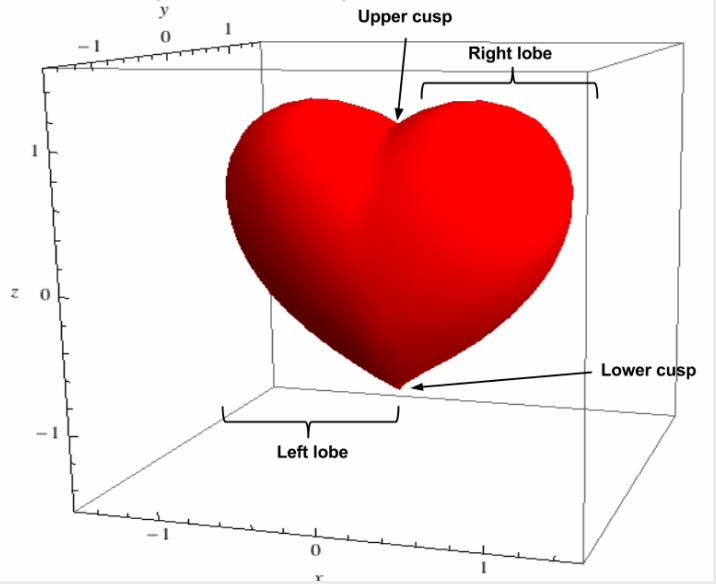
\includegraphics[trim=0.0cm 0.5cm 0.1cm 0.1cm, clip=true, totalheight=0.4\textheight]{Pictures/Heart.png}
\caption[Diagram of the heart-shaped primitive]{Diagram of the heart-shaped primitive}
\label{Heart}
\end{figure}

The   heart-­shape   was   stored   in   the   \textit{\textbf{include/}rtgeom.h}   file   as   an   Abstract   Data  
Type   ( C-­like   structure )   called   \textit{rt\_hrt\_internal}   with   the   following   fields  
representing its parameters.
\begin{itemize}  
\item A magic number \textit{\textbf{hrt\_magic }} 
\item A center point \textit{\textbf{v }} 
\item A vector in the direction of the X-­axis \textit{\textbf{xdir}}  
\item A vector in the directions of the Y­-axis \textit{\textbf{ydir}}  
\item A vector in the direction of the Z­-axis \textit{\textbf{zdir}}  
\item Distance from center point to either cusps \textit{\textbf{d}} 
\end{itemize} 
These   3    vectors viz \textit{\textbf{xdir}}, \textit{\textbf{ydir}} and \textit{\textbf{zdir}}   are   also   called   radial   vectors   because   they   radiate   in   the  X,   Y   and   Z   directions   and   the   aforementioned   structure   is   also   known   in  BRL-­CAD's parlance as the heart-­shape's internal format.

\subsection{A bare bones heart­-shape}

The   signatures   of   the   functions   which   are   called   to   compute   the  
geometric   properties   for   the   heart-­shaped   primitive   were   casted   and   enlisted   in  
a   function   table   in   \textit{src/librt/primitives/table.c}.   Then,   we   added   the  
\textit{src/librt/primitives/hrt/}   directory   to   the   source   code   repository   and   committed  
the   hrt.c   file   to   it.   The   hrt.c   file   consisted   of   introductory   comments,   include  
files,   structures   for   raytracing   and   storage   of   the   heart­-shaped   primitive   in   the  
database   as   well   as   stubs   for   all   callback   functions   which   all   print   a  
\textit{\textbf{\“rt\_hrt\_???:Not   implemented   yet!\”}}   message   when   called.   For   surface  
representation   and   raytracing   reasons,   the   heart-­shape   is   stored   in   a   more  
elaborate C-­like structure called \textit{hrt\_specific} with the following parameters;  

\begin{itemize}
\item A position vector for the heart-shape's center \textbf{\textit{hrt\_V}}  
\item A unit vector in the X ­axis direction \textbf{\textit{hrt\_X}}  
\item A unit vector in the Y axis direction \textbf{\textit{hrt\_Y}}  
\item A unit vector in the Z axis direction \textbf{\textit{hrt\_Z}}  
\item A unit vector in the Z ­axis direction \textit{\textbf{hrt\_d}}  
\item A matrix for scaling and rotating \textit{\textbf{hrt\_SoR}}  
\item A matrix for scaling and transposing a rotated heart \textbf{\textit{hrt\_invRSSR}}  
\item A matrix for transposing a rotated heart \textit{\textbf{hrt\_invR}}  
\item A vector for the inverse of the squared magnitudes of the three (3) aforementioned unit vectors \textit{\textbf{hrt\_invsq}}  
\end{itemize}

The   location   of   the   hrt.c   file   in   the   raytracing   library   was   added   to  
\textit{src/librt/CMakeLists.txt} for compilation purposes  and test ­driven development.\\
   
\hspace{30} After   hooking   the   heart-­shaped   primitive   into   BRL-­CAD's   source   code  
repository,   we   wrote   callback   functions   which   compute   geometrically   useful  
properties for the primitive such as;   

\begin{enumerate}
\item Formatted description  
\item Database importation and exportation  
\item Computing the bounding box of the heart­-shaped primitive  
\item Plotting the wireframe of the heart­-shaped primitive  
\item Implicit surface representation of the heart-­shaped primitive  
\end{enumerate}

\hspace{30} We   now   explain   how   the   functions   we   wrote   actually   compute   each
of   these properties.   Each   property   was   tested   using   BRL-­CAD's   commands \cite{36}   after  having   
written   the   requisite   function(s)   that   compute   it.   It   is   worth   highlighting  
here   that   the   \textit{“rt\_hrt\_”}   prefix   is   attached   to   the   heart­-shaped   primitive's   structure  
and   its   functions'   signatures   because   \textit{“rt”}   and   \textit{“hrt”}   denote   the   raytracing   library  
and the heart-shape respectively.  

\subsection{Formatted description of the heart­-shaped primitive}

\hspace{30} It   often   arises   that   engineers   and   scientists   working   on   geometric   models  
ask   to   know   the   exact   values   of   the   objects   in   question.   In   order   to   know   a  
solid's   type   and   the   values   of   its   key   parameters,   we   wrote   the   \textit{rt\_hrt\_describe()}  
function   which   simply   prints   the   heart-shape's   parameters   in   human   readable   format.  
The   radial   vectors   in   the   X,   Y   and   Z   directions   are   printed   alongside   their  
magnitudes   and   the   distance   from   the   heart-shape's   center   to   either   of   its   cusps   is  
also printed.

\subsection{Database importation and exportation of the heart­-shaped primitive}

\hspace{30} BRL-­CAD   provides   CSG   modeling   features   and   its   models   are   usually  
stored   in   it's   Geometric   Editing   database   called   GED.   For   the   heart­shaped  
primitive   to   be   used   in   CSG,   we   wrote   functions   that  
import and export data in between the database format and the internal format. 
  
The   \textit{rt\_hrt\_import5()}   function   imports   a   heart   from   the   database   format   to   the  
internal   format.   Firstly,   we   check   that   the   primitive   being   imported   is   the  
heart-­shaped   primitive   by   verifying   that   the   primitive's   magic   number   is   the  
same   as   the   heart-­shape's.   Then,   this   function   assigns   integers   held   in   an   array  
buffer to the different parameters of the \textit{rt\_hrt\_internal} structure.
   
We   wrote   the   \textit{rt\_hrt\_export5()}   function   to   export   the   heart­-shape's   internal  
format   into   the   database   format.   The   database   format   for   the   heart-­shape  
consists   rather   of   only   the   heart's   center   and   the   3   radial   vectors   in   the   X,   Y   and  
Z   directions.   It   is   not   really   useful   storing   value   for   d   in   the   database   as   it   is  
equivalent   to   some   components   of   the   radial   vectors.   After   checking   that   the  
primitive   in   question   is   the   heart,   we   store   the   values   for   \textit{v},   \textit{xdir},   \textit{ydir}   and   \textit{zdir} in an array buffer holding the integer values for the heart's parameters

\subsection{Computing the bounding box of the heart-­shaped primitive}

The   bounding   box   of   a   geometric   model   refers   to   the   box   with   the  
smallest   volume   within   which   the   model   lies   –   more   like   the   least   upper   bound  
of   the   set   of   all   enclosing   volumes.   The   spherical   equivalent   of   the   bounding  
box   is   the   bounding   sphere   which   is   the   smallest   sphere   within   which   a   model  
lies.   It   is   a   useful   property   to   compute   for   a   model   as   it   is   used   to   appropriately  
orient   an   object   (within   its   model   coordinates)   while   positioning   the   camera  
(within its world coordinates) and casting lights towards it.   

\hspace{30} In   order   to   compute   the   bounding   box   of   the   heart­-shape,   we   wrote   the  
\textit{rt\_hrt\_bbox()}   function   which   had   two   interesting   three­-dimensional   points   as  
parameters.   These   points   are   the   minimal   and   maximal   points   located   at   the  
closest   lower   left   hand   corner   and   the   furthest   upper   right   hand   corner   of   the  
bounding   box.   Obtaining   the   coordinates   of   these   two   points   suffices   to  
compute   the   bounding   as   they   are   located   at   opposite   ends   of   the   box,  
equidistant   from   the   heart-­shape's   center   and   differ   from   the   other   6   edges   by  
a single  component.  

\hspace{30} The   X   component   of   the   minimal   point   (closest   lower   left   hand   corner  
point)   is   obtained   by   subtracting   a   factor   of   2/3   from   the   unit   vector   from   the  
heart-­shape's   center.   The   X   component   of   the   maximal   point   (closest   lower   left  
hand   corner   point)   is   obtained   by   adding   a   factor   of   2/3   of   the   X   component   of  
the   unit   vector   to   the   heart-­shape's   center.

\hspace{30} The   Y   component   of   the   minimal  point   (closest   lower   left   hand   corner   point)
and   maximal   point   is   obtained   by  subtracting   and   adding   the   unit   vector   from   the   
heart-­shape's   center.   

\hspace{30} The   Z component   of   the   minimal   point   (closest   lower   left   hand   corner   point)   is  
obtained   by   subtracting   the   unit   vector   from   the   heart-­shape's   center   while   the   Z  
component   of   the   maximal   point   (furthest   upper   right   hand   corner   point)   is  
obtained   by   adding   another   factor   of   1.25   to   the   unit   vector   to   the   heart­-shape's  
center   in   a   component­wise   manner.   The   factor   of   1.25   in   the   calculation   of   the  
Z   component   of   the   maximal   point   represents   the   distance   from   the   heart's  
center   to   either   of   its   cusps   (which   is   1.0)   and   the   additional   0.25   closely  
approximates   the   displacement   from   the   upper   cusp   to   the   highest   point   on  
either   of   its   lobes.

With   the   coordinates   of   the   maximal   and   minimal   points  
obtained, we obtain the bounding box of the heart-­shape.  

\subsection{Plotting the wireframe of the heart-­shaped primitive}

\hspace{30} As   we   earlier   discussed,   the   wireframe   of   an   object   enables   the  
sketching   and   preview   of   objects   before   adding   colour   and   texture   to   them.   In  
order   to   build   the   wireframe   of   the   heart­shaped   primitive   into   BRL-­CAD's  
functionality,   we   wrote   the   \textit{rt\_hrt\_plot()}   and   \textit{rt\_hrt\_24pts()}   functions.   The  
heart-­shaped   primitive's   wireframe   is   made   up   of   several   ellipses   aligned   along  
the   Z   axis   each   of   which   consists   of   24   edges.   As   we   progress   in   the   positive  
 Z - ­axis   direction,   we   use   8   ellipses   (with   decreasing   radii)   to   frame   the   upper  
portions   of   the   left   and   right   lobes.   The   24   required   points   for   each   ellipse   are  
computed   by   the   \textit{rt\_hrt\_24pts()} function which computes 24 points which are $15^{\circ}$ apart.
Finally,   the   different   ellipses   are  connected   together   to   enrich   the   wireframe   
with   more   iso­contours.   Along   the  XY   and   XZ   planes   (when   Z   =   0   and   Y   =   0   respectively), the   heart-­shape's  wireframe   appears   like   an   ellipse.   Along   the   YZ   plane   (when   X   =   0),   the  
heart-­shape   primitive's   wireframe   is   indeed   heart­-shaped.   The   algorithm   below  
was used to develop the wireframe of the heart­-shape.  

\hspace{50} \textit{Algorithm 1. Plotting the wireframe of the heart­-shape }
\footnotesize{\begin{verbatim}
1. for points in the +Z directions starting at the upper cusp 
        locate centres of ellipses which constitute the upper half of the left lobe 
        determine radial vectors in X, Y and Z directions as need be 
        determine the 24 points for each ellipse 
        draw each ellipse        // Connect the 24 points 
        make connections between ellipses 
        end at highest point of left lobe         // the maximum turning point 
2. for points in the +Z directions starting at the upper cusp 
        locate centres of ellipses which constitute the upper half of the right lobe 
        determine radial vectors in X, Y and Z directions as need be 
        determine the 24 points for each ellipse 
        draw each ellipse        // Connect the 24 points 
        make connections between ellipses 
        end at highest point of right lobe         // the maximum turning point   
3. for chosen levels in the +Z direction starting at the lower cusp 
        locate centres of ellipses 
        determine radial vectors in X, Y and Z directions as need be 
        determine the 24 points for each ellipse 
        draw each ellipse        // Connect the 24 points 
        make connections between ellipses
        end at upper cusp level        //the maximum turning point 
\end{verbatim}}

\subsection{Surface   representation   and   raytracing   of   the   heart­-shaped primitive}

\hspace{30} The   heart-­shaped   primitive   endowed   with   a   surface   representation   by  
raytracing   it.   Ray­tracing   at   its   very   core   consists   of   solving   for   the   intersection  
points   of   a   line   and   a   surface.   Many   interesting   surfaces   have   been   written   as  
polynomial   functions   of   position   and   the   heart­-shape   is   not   left   out.   The  
peculiarity   of   our   work   is   that   we   proved   that   ray­tracing   using   the  
Laguerre­-based   root­finder   works   for   sextic   equations   (those   with   a   degree   of  
6).   In   order   to   do   this,   we   wrote   \textit{rt\_hrt\_prep()},   \textit{rt\_hrt\_norm()},   \textit{rt\_hrt\_shot()}   and  
\textit{rt\_hrt\_print()} functions.

\hspace{30} The   \textit{rt\_hrt\_prep()}   function   prepares   a   heart-­shape   for   ray­tracing   by  
verifying   that   the   object   in   question   is   a   valid   heart-­shape.   If   the   primitive   is   a  
valid   heart,   then   a   specific   heart   structure   called   \textit{hrt\_specific}   is   created   and  
stored   in   memory   for   use   by   the   \textit{rt\_hrt\_shot()}   function.   To   check   the   validity   of  
the   heart,   we   first   check   that   at least   one   of   the   three   radial   vectors   has   a  
positive   magnitude.   Secondly,   we   check   that   the   value   for   parameter   d   is  
non­zero   and   is   not   too   large.   After,   we   check   that   the   3   radial   vectors   are  
perpendicular   to   each other.   If   they   are   indeed   perpendicular   to   each   other,   then  
the   heart­-shaped   primitive   is   a   valid   hear.   Finally,   we   compute   values   for   \textit{d},   \textit{v},  
\textit{hrt\_invRSSR},   \textit{hrt\_invsq}   and   the   heart-shape's   bounding   sphere   centered   at   \textit{v}.   After  
computing   these   requisite   parameters   for   the   heart   in   \textit{rt\_hrt\_prep()},   the  
\textit{rt\_hrt\_print()}   function   prints   the   position   vector   of   the   heart-­shape's   center   and  
the   two   (2)   matrices   for   transposing,   rotating   and   scaling   just   to   make   sure   that  
are correct.

\hspace{30} Millions   of   light   rays   are   shot   at   the   surface   of   the   heart   and   the   pixels  
where   intersections   occur   are   rendered.   The   \textit{rt\_hrt\_shot()}   function   came   in  
handy   at   this   point   of   our   development   of   the   heart-­shape.   Each   point   in $ \mathbb{E}^3 $
   is   represented   by   a   treble   (x,y,z)   and   the heart-­shaped   primitive's   surface   is   implicitly   represented   as   a   sextic   equation as shown in (6) below.  

\begin{equation*}
\centering
  ­­­­­­­­­­­­­­f(x,y,z) = {(x^2 + 9/4y^2 + z^2 - 1 )}^3 - z^3(x^2 + 9/80y^2) \tag{6}
\end{equation*}

Each   light   ray   is   modeled   as   a   line   in   $ \mathbb{E}^3 $   written  
as   a   linear   equation   written   in   the   form   $W   =   Dt   +   P$   where   W   =   (x,y,z),   D   =   (a,b,c),  
P   =   ($x_0,y_0 ,z_0$) and $a$,$ b$, $ c$,$x_0$,$y_0$ and $z_0$ are constants in $ \mathbb{R} $.   The   system   of  
equations for the components of W is given below

\begin{IEEEeqnarray*}
\centering
x = at + $x_0$ \\
y = bt + $y_0$ ­­­­­­­­­­­­­­­­­­­­­­­­­­­­­\IEEEyesnumber \\
z = ct + $z_0$ \\
\end{IEEEeqnarray*} 

This   equation   (6)   indicates   that   each   point   on   the   line   is   represented   by   a  
unique   value   for   t.   To   find   the   points   of   intersection   of   the   light   ray   and   the  
surface   of   the   heart-­shaped   primitive,   we   substituted   x,   y   and   z   from   (6)   above  
into equation (5). This yielded a new sextic equation (7) in t shown below
\begin{equation*}
\centering
S(t) = C_6t^6  + C_5t^5 + C_4t^4 + C_3t^3 + C_2t^2 + C_1t + C_0  = 0 ­­­­­ \tag{7}  
\end{equation*}
where   Ci,i = 0$\div$6 are the coefficients of equation (7) which can be viewed in the Appendix.

The   real   zeroes   of   (7)   indicate   an   intersection   in $ \mathbb{E}^3 $.
Even   if   complex   roots   are   returned   by   the   root­finder,   the   roots   with  
imaginary   components   sufficiently   close   to   zero   are   considered   to   be   real  
zeroes   and   are   also   used   as   values   for   t   in   intersection   points. 
If   there   are   no  real   solutions,   then   the   ray   does   not   intersect   the   heart's   surface.   We   determine  
the   coordinates   of   the   intersection   points   by   substituting   the   values   for   real   $t_i$ in $ W $ above.  

The   Algorithm   below   shows   the   intersection   of   an   arbitrary   light   ray   and   the  heart­-shape's surface.

\hspace{50} \textit{Algorithm 2. Intersect a ray with the heart­-shape's surface }
\small{\begin{verbatim}
Normalize distance from the heart-­shape 
Generate sextic equation 
Pass equation through Laguerre-­based root finder  
if (root finder returns other than 6 roots) 
    throw exceptions	  // root finder did not find roots 
else         	// Real roots indicate an intersection in real space 
    select real roots among the 6 //complex roots with very small imaginary parts 
for each real root returned by root finder 
       Determine the entry and exit points of the light ray 
\end{verbatim}}

\hspace{30} The   normal   to   the   surface   $N$   at   the   point   of   intersection   is   in   the   direction  
of   the   gradient   of   \textit{f(x,y,z)}. N := ($f_x$,$f_y$,$f_z$)   where   $f_x$, $f_y$ and $f_z$   are   the   partials  
derivative   functions   of   \textit{f(x,y,z)}   with   respect   to   x,   y   and   z   respectively.   The  
function   \textit{rt\_hrt\_norm()}   computes   the   surface   normal   N   to   the   surface   of   the  heart-­shaped primitive.

By substituting   $w = x^2 + 9/4y^2 + z^2 – 1$,   (6)   becomes   

\hspace{100} $w^3 – z^3(x^2 + 9/80y^2) = 0$ 

and the surface normal is given by the system of equations in below.

\begin{IEEEeqnarray*}
\centering
$f_x(x,y,z)$ = 6x(w^2 – z^3/3) \\
$f_y(x,y,z)$ = 6y(12/27w^2 – 88/3z^3) ­­­­­­­­­­­­­­­­­­­­­­­­­­­­­\IEEEyesnumber \\
$f_z(x,y,z)$ = 6z(w^2 – z/2(x^2 + 9/80y^2))   \\
\end{IEEEeqnarray*}

\hspace{30} Computing   the   exact   algebraic   expression   for   the   coefficients   of   (7) above   is  
cumbersome   and   error-­prone.   Instead,   we   use   several   polynomial   variables   to  
hold   the   coefficients   of   (7)   and   gradually   build   equation   (7).   Starting   with  
polynomials   for   $x^2$, $9/4y^2$ and $z^2 ­- 1$,   we   obtain   w. With   $y^2$ + $9/4x^3$   and   $z^3$ ,   we  
obtain $z^3(x^3 + 9/80x^3)$. Hence, we obtain coefficients of (7). 

\hspace{30} Once   the   coefficients   of   (7)   are   determined,   it   is   parsed   through  
BRL­-CAD's   root   finder.   For   polynomials   with   degrees   less   than   five,   there  
exists   exact   solutions   in   radicals.   Indeed,   linear   and   quadratic   equations   can   be  
trivially   solved   by   the   substitution   method   and   the   quadratic   formula  
respectively.   A   method   for   solving   cubics   was   discovered   by   Cardan   and   a  
method   for   solving   quartics   was   discovered   by   Ferrari.   Although   some  
methods   exist   to   determine   the   exact   solutions   of   higher   order   polynomials  
(with   degrees   greater   than   4)   in   radicals   from   Galois   theory,   the   equation   (7)  
does   not   satisfy   these   conditions.   Indeed,   the   Galois   group   of   equation   (7)   is  
contained   neither   in   the   group   of   order   48   which   stabilizes   a   partition   of   the   set  
of   the   roots   into   three   subsets   of   two   roots   nor   in   the   group   of   order   72   which  
stabilizes   a   partition   of   the   set   of   the   roots   into   two   subsets   of   three   roots.   As   a  
result, only numerical methods can be employed to solve it.  
 
Fortunately,   BRL-­CAD   has   a   root­solver   which   is   based   on   a   numerical  
method   called   the   Laguerre   method.   Named   after   the   French   mathematician  
Edmund   Laguerre,   the   Laguerre   method   is   a   root­finding   algorithm   used   to  
solve   polynomials.   Extensive   empirical   studies   show   that   this   method   has   come  
close   to   being   a   sure­fire   method   because   it   almost   always   converges   to   some  
root   of   the   polynomial   no   matter   what   initial   guess   is   chosen.   This   is   in   contrast  
to   the   other   methods   like   the   Newton­-Raphson   method   which   may   fail   to  
converge   for   poorly   chosen   initial   guesses.   Algorithm   3   below   shows   how   the  
Laguerre method works;  

\hspace{85} \textit{Algorithm 3. The Laguerre Root­-finding Method  }

1. Choose an initial guess $x_0$  \\
2. while (k < N or a is not sufficiently small) \\
\hspace{10}2.1. for k = 0$\div$N \\
\hspace{30}Compute  G := f'($x_k$)/f($x_k$) \\ 
\hspace{30}Compute  H := G^2 – f''($x_k$)/f($x_k$) \\ 
\hspace{30}Compute  a := $n/G + \sqrt{(n–1)(nH – G^2f(x))}$ ,n = degree of f(x) \\
\hspace{10}end for loop \\
\hspace{10}2.2 Set $x_{k+1}$ := $x_{k – a}$\\ 
end while loop \\

If   a   root   is   found,   then   the   corresponding   linear   factor   is   removed   from   the  
polynomial.   This   deflation   step   reduces   the   degree   of   the   polynomial   by   one  
and approximations for all roots of the polynomial are obtained. 
 
\hspace{30} BRL-­CAD's   root­finder   \textit{rt\_poly\_findroot()}   function   is   found   in  
\textit{\textbf{src/librt/roots.c}}.   We   tested   the   root   solver   to   show   that   it   solves   sextic  
equations by parsing an arbitrarily chosen equation (8) below  

\begin{equation*}
\centering
 x^6 -­ 8x^5 + 32x^4 - 78x^3 + 121x^2 - ­110x + 50 = 0­­­­­ \tag{8}  
\end{equation*}
Equation (8) is parsed through the   root­finder   to   obtain   its   roots   $x_1 = 1 – i$, $x_2 = 1 + i$, $x_3 = 2 – i$, $x_4 = 2 +
i$, $x_5 = 1­ - 2i$, $x_6 = 1 + 2i$. This   test   is   implemented   in   \textit{\textbf{src/util/roots\_example.c}}.  
Besides   this   test,   the   call   to   the   root­finder   by   (6)   worked   and   rendered   the  
heart-shape as our discussion of results in the next chapter will show.  

\subsection{Type in support for the heart-­shaped primitive}

Finally,   appropriate   support   for   typing   the   parameters   of   the   heart­-shaped  
primitive   using   the   keyboard   into   the   mged   or   archer   interfaces   was  
implemented.   To   do   this,   we   first   wrote   the   \textit{p\_hrt[]}   array   and   \textit{hrt\_in()}   routine   in  
\textit{\textbf{src/libged/typein.c}}   to   prompt   users   to   input   parameters   for   the   heart­-shape.  
Then ,we   added   the   \textit{mk\_hrt()}   function   to   the   include/wdb.h   and  \textit{\textbf{src/libwdb/wdb.c}} files   to   assign   values   from   \textbf{mged}   or   \textbf{archer}   interfaces   to   the  heart-shape's parameters.


\hspace{30} In   this   chapter,   we   introduced   the   concept   of   open   source   software  
because   our   research   was   carried   out   within   this   context.   Secondly,   we   described  
the   procedure   for   constructing   the   heart­-shaped   primitive. After, we   outlined   the  
design   of   the   heart­-shaped   primitive   and   the   implementation   of   appropriate  
callback   functions   to   compute   geometrically   important   properties   for   the  
heart­-shape.  
%-----------------------------------------------------------------------------------------------------------------------------------
